\section{Introduction}

Deep Reinforcement Learning (Deep-RL) is starting to achieve interesting results in different areas such as tasks involving the control on discrete systems \cite{mnih2013playing}, \cite{schaul2015prioritized} continuous systems \cite{lillicrap2015continuous}, \cite{schulman2015high}, \cite{nachum2017trust}
and more recently in robotics \cite{gu2017deep}, \cite{mahmood2018benchmarking}, \cite{richter2019open}.
The first applications of deep reinforcement learning in robotics were in the use of manipulation in a  fully observable and stable environment \cite{gu2016continuous} but tasks in mobile robotics involving obstacles interacting with physical environments and objects, turns the workplace more complex.
In order to overcome this problem, Deep-RL methods normally try to discretize the actions to turn simpler the problem \cite{zhu2017target}, \cite{tai2016towards}.
Recent articles explore continuous control actions used for navigation of mobile robots with good results \cite{tai2017virtual}, \cite{chen2017socially}.

In this paper, we try to demonstrate how effective can be the Deep-RL in mobile robotics, in order to achieve that we explore the use of Deep-RL in a simulator and in a real robot.
For the simulator, two environments were used on Gazebo. 
The simulator can provide us with a lot of resources for robot simulation, for example, we can create an environment and insert a model of a real mobile robot \cite{fairchild2016ros}, \cite{joseph2015mastering}. 
The mobile robot used on the simulation was the Turtlebot3.

The objective of this research is to show the efficiency of a Deep-RL network in the task of mobile robot navigation from an initial position to a target on an environment.
To simplify this problem it was created a network which has 14 inputs and 2 outputs, as shown in Fig. \ref{fig:mapless}.
The 14 inputs are composed by 10 readings of the laser sensor, the previous linear and angular velocity, the distance and angle of the mobile robot related to the target.
And the outputs of the network are the linear and angular velocity that are sent to the robot in order to get to the target.
It is expected that the intelligent agent will not collide with any obstacle on its trajectory to the target.

\begin{figure}[htbp]
\centerline{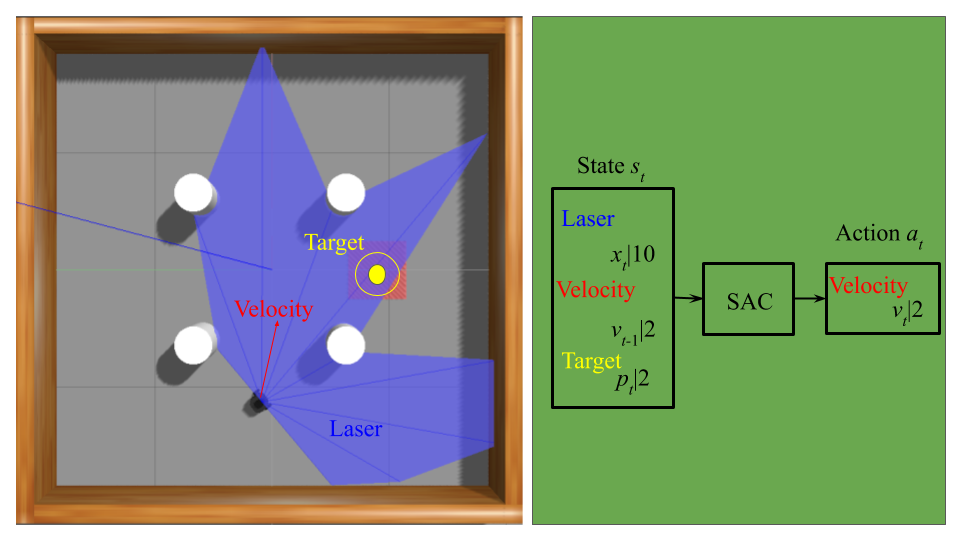
\includegraphics[width=\columnwidth]{images/mapless.png}}
\caption{System definition.}
\label{fig:mapless}
\end{figure}

This work is divided in seven sections.
After a brief introduction in the first section of the Deep-RL on the mobile robot navigation, the second section describes the work of authors on the field that inspired this research, the third section gives a background about the used technique, the fourth section makes an introduction of the tools used for the project, the fifth section summarizes the methods so that the robot can get to a target, the sixth section presents the results obtained on the Gazebo environments, the seventh section makes the discussion on the results and applications of Deep-RL.